\documentclass[11pt]{article}
\usepackage[margin=0.95in]{geometry}
\usepackage{amsmath,amssymb}
\usepackage{graphicx}
\usepackage{booktabs,longtable,array}
\usepackage{xcolor}
\usepackage[hidelinks]{hyperref}
\usepackage{enumitem}
\usepackage{caption}
\setlist{itemsep=2pt,topsep=4pt}
\captionsetup{font=small,labelfont=bf}
\setlength{\parskip}{5pt}
\setlength{\parindent}{0pt}
\renewcommand{\arraystretch}{1.15}
\title{Stage T2: Does the Actor Learning Rate Explain TRM's TD3 Failure?}
\author{}
\date{trm-delay-robust-scaling $\cdot$ Phase 5 stage note $\cdot$ 2026-10-10\\[2pt]Plan \texttt{.\allowbreak{}.\allowbreak{}/\allowbreak{}plan/\allowbreak{}plan.\allowbreak{}md} \S{}2 (frozen 2026-10-10, before any Phase 5 data); gate GT2 and amendment P5-1 in \texttt{.\allowbreak{}.\allowbreak{}/\allowbreak{}.\allowbreak{}.\allowbreak{}/\allowbreak{}experiments/\allowbreak{}phase5/\allowbreak{}gates.\allowbreak{}json}; analysis in \texttt{.\allowbreak{}.\allowbreak{}/\allowbreak{}.\allowbreak{}.\allowbreak{}/\allowbreak{}experiments/\allowbreak{}analysis\_\allowbreak{}p5\_\allowbreak{}t2.\allowbreak{}json}; exploratory numbers in \texttt{figures/\allowbreak{}derived\_\allowbreak{}numbers\_\allowbreak{}p5.\allowbreak{}json}.}
\begin{document}
\maketitle
\section*{1. Question and rule}



Phase 4's Stage T reran Phase 3's capacity contrast under TD3 with \texttt{conf/\allowbreak{}arch/\allowbreak{}td3.\allowbreak{}yaml} unchanged. Its gate GT passed (TRM 788k $-$ MLP 788k negative in 12/12 pairs), but \texttt{gates.json} records a caveat with it: the pass reflected an optimisation failure. TRM 788k stayed at random-policy level in 10 of 12 runs and its critic loss rose through training, while every MLP run learned. The caveat named a likely contributor, untested: \texttt{td3.yaml}'s actor learning rate of 1e-3 is ten times the DDPG actor rate (1e-4) under which TRM trained normally in Phases 1--4. Stage T2 tests that directly.



\begin{itemize}
\item \textbf{Design.} Pendulum-v1, TD3 with \texttt{td3.yaml}, only \texttt{arch.actor\_lr} overridden: critic LR 1e-3, batch 256, warmup 10,000 steps and policy delay 2 are unchanged. 200 episodes. Conditions C0 (no delay) and C1 (fixed d = 1 with the one-slot queue, no previous-action input), the two Stage T used. Seeds 1--6.
\item \textbf{Arms.} TRM 788k (\texttt{trm}) at actor LR 1e-4 and 3e-4 (12 runs each); TRM 788k at 1e-3, which is Stage T's 12 runs reused under amendment P5-1; and a control, MLP 788k (\texttt{dnn\_large}) at actor LR 1e-4 (12 runs). 36 new jobs.
\item \textbf{"Learned"} means final avg-100 > $-$1000, fixed before any data. Stage T had used the same cut descriptively. A uniform-random policy scores $-$1163.84 (Phase 4 amendment R-2).
\end{itemize}



\begin{quote}\textbf{Gate GT2.} For each actor LR, report TRM 788k runs learned out of 12. \textbf{"LR explains the TD3 failure"} if TRM 788k learns in $\geq$ 10/12 runs at some actor LR < 1e-3. If it does, also report TRM 788k $-$ MLP 788k at that LR (n = 12 (seed, condition) pairs, sign test, two-sided p). If both 1e-4 and 3e-4 pass, both contrasts are reported: the 1e-4 one is LR-matched and primary; the 3e-4 one compares unequal actor LRs and is labelled so. \emph{Secondary:} late critic-loss medians (last quarter of episodes), eval last-5, and the control MLP's learned count against Stage T's MLP 788k at actor LR 1e-3.\end{quote}



\textbf{Amendment P5-1} (2026-10-10, before data, author-approved). The TRM arm at 1e-3 reuses Stage T's runs: same configuration, code verified byte-identical to the frozen Stage T snapshot \texttt{p4code/t}. Runs are not bit-reproducible across GPU models, which \texttt{gates.json} records as the caveat on the reuse.



\textbf{Parameter counts} (actor + twin critics, excluding targets, from each run's \texttt{param\_count}): TRM 788k 1,181,443 (C0) and 1,181,827 (C1); MLP 788k 1,180,611 and 1,182,483. The "788k" labels name the DDPG-basis configurations, as in Stage T.



\section*{2. Results}



\textbf{Arms} (12 runs each: 6 seeds $\times$ 2 conditions).



\begin{center}\small\begin{tabular}{>{\raggedright\arraybackslash}p{0.238\linewidth}>{\raggedright\arraybackslash}p{0.079\linewidth}>{\raggedleft\arraybackslash}p{0.119\linewidth}>{\raggedleft\arraybackslash}p{0.119\linewidth}>{\raggedleft\arraybackslash}p{0.109\linewidth}>{\raggedleft\arraybackslash}p{0.158\linewidth}}
\toprule
Arm & Actor LR & Runs learned & Median final & Eval last-5 & Late critic loss \\
\midrule
TRM 788k & 1e-4 & \textbf{12/12} & $-$187.69 & $-$173.08 & 36.01 \\
TRM 788k & 3e-4 & \textbf{11/12} & $-$234.56 & $-$200.71 & 47.36 \\
TRM 788k (Stage T, P5-1) & 1e-3 & 2/12 & $-$1389.27 & $-$1415.09 & 560.94 \\
MLP 788k (control) & 1e-4 & 12/12 & $-$176.14 & $-$167.98 & 25.37 \\
MLP 788k (Stage T) & 1e-3 & 12/12 & $-$175.92 & $-$168.25 & 23.69 \\
\bottomrule
\end{tabular}\end{center}



\emph{Source: \texttt{experiments/\allowbreak{}analysis\_\allowbreak{}p5\_\allowbreak{}t2.\allowbreak{}json} (\texttt{arms}). Final = final avg-100 training return; late critic loss = median over the last quarter of episodes.}



\textbf{Contrasts} (n = 12 (seed, condition) pairs).



\begin{center}\small\begin{tabular}{>{\raggedright\arraybackslash}p{0.319\linewidth}>{\raggedright\arraybackslash}p{0.147\linewidth}>{\raggedleft\arraybackslash}p{0.069\linewidth}>{\raggedleft\arraybackslash}p{0.081\linewidth}>{\raggedleft\arraybackslash}p{0.092\linewidth}>{\raggedleft\arraybackslash}p{0.115\linewidth}}
\toprule
Contrast & Label & Median $\Delta$ & Mean $\Delta$ & Positive & p (two-sided) \\
\midrule
\textbf{TRM 788k @ 1e-4 $-$ MLP 788k @ 1e-4} & \textbf{LR-matched (primary)} & \textbf{$-$12.98} & $-$14.45 & \textbf{2/12} & \textbf{0.039} \\
TRM 788k @ 3e-4 $-$ MLP 788k @ 1e-4 & unequal actor LRs & $-$53.60 & $-$159.41 & 0/12 & 0.0005 \\
\emph{Reference:} TRM 788k $-$ MLP 788k, DDPG (Phase 3 G1) & --- & $-$27.14 & $-$29.85 & 2/12 & 0.039 \\
\bottomrule
\end{tabular}\end{center}



\emph{Source: \texttt{experiments/\allowbreak{}analysis\_\allowbreak{}p5\_\allowbreak{}t2.\allowbreak{}json} (\texttt{contrasts}); Phase 3 reference from \texttt{experiments/\allowbreak{}analysis\_\allowbreak{}s1.\allowbreak{}json} (\texttt{large: trm - dnn\_\allowbreak{}large}).}



\textbf{GT2: "LR explains"}, as recorded in \texttt{gates.json}. TRM 788k learned in 12/12 runs at actor LR 1e-4 and 11/12 at 3e-4, against 2/12 at 1e-3; both lower rates clear the $\geq$ 10/12 bar. The control MLP learned 12/12 at 1e-4, as Stage T's MLP did at 1e-3. At the LR-matched setting, TRM 788k $-$ MLP 788k is $-$12.98 (2/12 positive, two-sided p = 0.039).



\begin{figure}[htbp]\centering
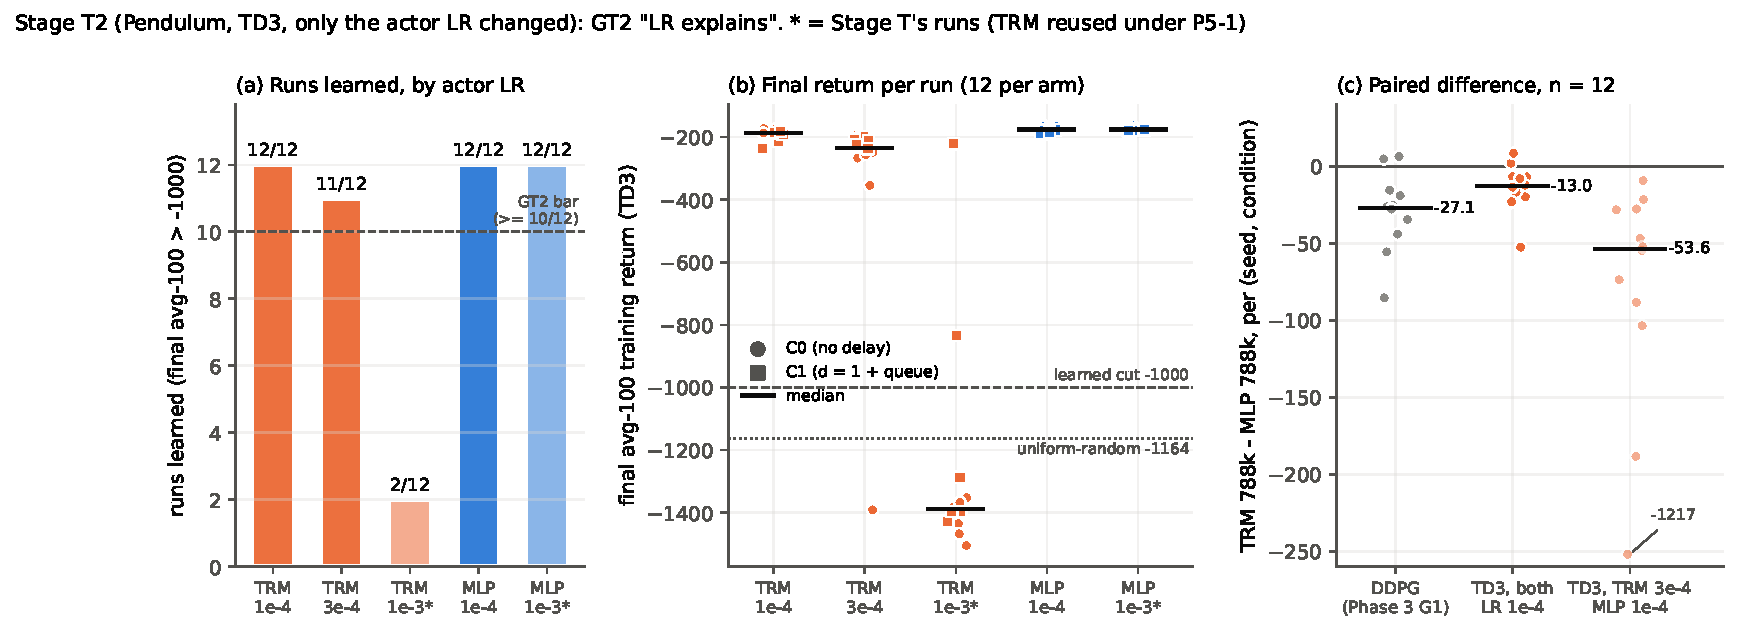
\includegraphics[width=\linewidth,height=0.42\textheight,keepaspectratio]{figures/p5_f1_t2_learned_finals.pdf}
\caption{Stage T2: runs learned and final return per run by actor LR, and the paired TRM $-$ MLP difference against Phase 3's DDPG contrast}
\end{figure}



\begin{figure}[htbp]\centering
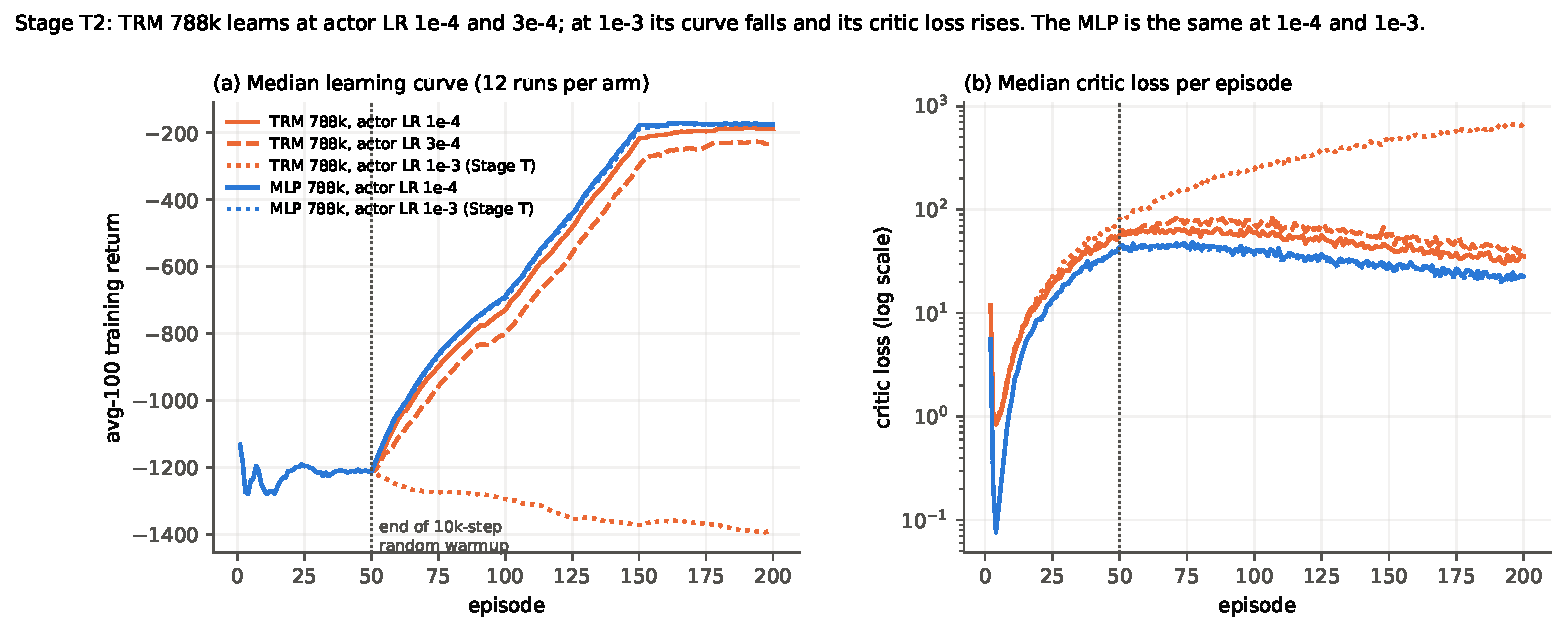
\includegraphics[width=\linewidth,height=0.42\textheight,keepaspectratio]{figures/p5_f2_t2_curves.pdf}
\caption{Stage T2: median learning curves and critic loss per episode, by arm}
\end{figure}



\textbf{Secondary and exploratory numbers} (computed from the raw results by \texttt{make\_\allowbreak{}figures\_\allowbreak{}phase5.\allowbreak{}py}; not part of the gate).



\begin{center}\small\begin{tabular}{>{\raggedright\arraybackslash}p{0.193\linewidth}>{\raggedleft\arraybackslash}p{0.122\linewidth}>{\raggedleft\arraybackslash}p{0.122\linewidth}>{\raggedleft\arraybackslash}p{0.136\linewidth}>{\raggedleft\arraybackslash}p{0.122\linewidth}>{\raggedleft\arraybackslash}p{0.129\linewidth}}
\toprule
Quantity & TRM 1e-4 & TRM 3e-4 & TRM 1e-3 (Stage T) & MLP 1e-4 & MLP 1e-3 (Stage T) \\
\midrule
Learned, C0 / C1 & 6/6, 6/6 & 5/6, 6/6 & 0/6, 2/6 & 6/6, 6/6 & 6/6, 6/6 \\
Median final, C0 / C1 & $-$180.78 / $-$190.31 & $-$261.53 / $-$217.82 & $-$1408.96 / $-$1341.56 & $-$168.00 / $-$181.51 & $-$168.94 / $-$177.51 \\
Critic loss, episodes 51--75 & 59.2 & 68.5 & 118.6 & 44.0 & 41.2 \\
Critic loss, last quarter & 36.0 & 47.4 & 560.9 & 25.4 & 23.7 \\
Runs where late > early & 0/12 & 2/12 & 11/12 & 0/12 & 0/12 \\
\bottomrule
\end{tabular}\end{center}



\emph{Source: \texttt{figures/\allowbreak{}derived\_\allowbreak{}numbers\_\allowbreak{}p5.\allowbreak{}json} (\texttt{t2.per\_arm}).}



\begin{center}\small\begin{tabular}{>{\raggedright\arraybackslash}p{0.483\linewidth}>{\raggedleft\arraybackslash}p{0.069\linewidth}>{\raggedleft\arraybackslash}p{0.189\linewidth}>{\raggedleft\arraybackslash}p{0.137\linewidth}}
\toprule
Paired quantity (n = 12) & Median & Positive / above 1 & p (two-sided) \\
\midrule
Late critic loss ratio, TRM @ 1e-4 / MLP @ 1e-4 & 1.50$\times$ & 12/12 & --- \\
Late critic loss ratio, TRM @ 3e-4 / MLP @ 1e-4 & 1.75$\times$ & 12/12 & --- \\
Eval last-5, TRM @ 1e-4 $-$ MLP @ 1e-4 & $-$6.68 & 2/12 & 0.039 \\
Final, MLP @ 1e-4 $-$ MLP @ 1e-3 (Stage T) & $-$0.03 & 6/12 & 1.00 \\
Final, TRM @ 1e-4 $-$ TRM @ 3e-4 & +37.89 & 10/12 & 0.039 \\
\bottomrule
\end{tabular}\end{center}



\emph{Source: \texttt{figures/\allowbreak{}derived\_\allowbreak{}numbers\_\allowbreak{}p5.\allowbreak{}json} (\texttt{t2.pairs}). For comparison, the late critic-loss ratio TRM 788k / MLP 788k was 1.89$\times$ (12/12) under DDPG in Phase 3 and 24.91$\times$ (12/12) in Stage T (\texttt{analysis\_\allowbreak{}p4\_\allowbreak{}t.\allowbreak{}json}).}



\section*{3. What the numbers show}



\begin{itemize}
\item \textbf{The TD3 failure goes away when only the actor learning rate is lowered.} At 1e-4 every TRM 788k run learns, at both conditions; its median learning curve rises after warmup like the MLP's instead of falling. At 3e-4 eleven of twelve learn; the one that does not is C0, seed 1 (final $-$1391.2).
\item \textbf{The critic divergence goes with it.} At 1e-3 TRM's critic loss rose from 118.6 (episodes 51--75) to 560.9 (last quarter), in 11/12 runs. At 1e-4 it falls, from 59.2 to 36.0, in every run, as the MLP's does. The critic's own learning rate (1e-3) was the same in all arms, so the divergence was set off by the actor's step size, not the critic's.
\item \textbf{At the LR-matched setting TRM still trails the MLP, by a modest and consistent margin.} TRM 788k $-$ MLP 788k is negative in 10 of 12 pairs, median $-$12.98. The two positive pairs are C0 seed 1 (+2.01) and C1 seed 5 (+8.38). This is the same direction and the same sign count (2/12) as Phase 3's G1 contrast under DDPG ($-$27.14); the median is about half as large. TRM's late critic loss is above the MLP's in all 12 pairs (1.50$\times$), as it was under DDPG (1.89$\times$).
\item \textbf{The deficit is small on the greedy policy too, but consistent.} On eval last-5 TRM @ 1e-4 trails by a median 6.68 (2/12). One pair (C1 seed 5) has a $-$176.48 eval difference although its training-return difference is positive; the median is not driven by it.
\item \textbf{The MLP does not care about the actor rate; TRM does.} MLP 788k at 1e-4 and at 1e-3 differ by a median $-$0.03 (6/12), with nearly identical medians, eval and critic loss. TRM goes from 12/12 learned at 1e-4 to 11/12 at 3e-4 to 2/12 at 1e-3, and even between 1e-4 and 3e-4 it loses a median 37.89 (10/12 pairs favour 1e-4). Phase 4's Stage C found the same direction under DDPG: all three $\times$3-actor-LR cells (3e-4) were below the default in 3/3 seeds.
\item \textbf{Cost is unchanged.} On L40S GPUs the median TRM 788k run at 1e-4 took 22.69 min (9 runs) against the MLP's 2.04 min (12 runs), 11.1$\times$. Stage T's longer TRM median (42.54 min) reflects its hardware mix (7 of 12 runs on V100); its one L40S run took 23.37 min.
\end{itemize}



\section*{4. What the result does and does not settle}



\textbf{It settles the open question GT left.} The caveat in Phase 4's \texttt{gates.json} named the actor LR as the likely, untested contributor; GT2 tests it and the answer is yes. GT's status in Phase 4's \texttt{gates.json} is unchanged ("pass"); what changes is its interpretation. With a DDPG-like actor rate TRM trains under TD3 and the capacity contrast shows a Phase-3-like deficit rather than a failure to train. Phase 3's attribution, that TRM trails a parameter-matched MLP for architectural reasons, now holds under two algorithms at matched, sensible learning rates.



\textbf{It does not settle:}



\begin{itemize}
\item \emph{Whether 1e-4 is TRM's best TD3 actor rate.} The grid has three points. A lower rate was not tried, so the size of the deficit at TRM's best TD3 setting is not measured (plan threat 2).
\item \emph{Which part of the actor step causes the collapse.} The actor update and the critic's divergence cannot be separated here; the result shows only that the critic diverges when, and only when, the actor rate is high.
\item \emph{Why TRM is so much more LR-sensitive than the MLP.} That is an observation (exploratory), not a tested mechanism.
\item \emph{Anything beyond Pendulum-v1.}
\end{itemize}



\section*{5. Threats to validity}



\begin{enumerate}
\item \textbf{The learned threshold is coarse.} $-$1000 separates runs that learned from runs near random ($-$1163.84), not good runs from mediocre ones. The gate result is not sensitive to it here: every TRM run at 1e-4 ends between $-$171.7 and $-$237.4, and the one failed 3e-4 run ends at $-$1391.2.
\item \textbf{Three LR points.} A pass shows the failure is LR-sensitive, not that 1e-4 is optimal.
\item \textbf{The MLP control ran at one new LR.} The 3e-4 contrast mixes architecture with learning rate and is labelled so. The MLP's insensitivity between 1e-4 and 1e-3 makes it unlikely that a different MLP rate would change the comparison much, but that is an inference across stages.
\item \textbf{Cross-GPU reproducibility.} Runs are not bit-reproducible across GPU models (Phase 4 B0). Every new MLP run ran on an L40S; the new TRM runs ran on L40S (15), V100 (4), H100 (3) and A100 (2); the reused 1e-3 arm ran mostly on V100 and A100. Hardware variation is part of the seed variation in every contrast.
\item \textbf{Reuse (P5-1).} The 1e-3 arm was submitted on 2026-10-07 (\texttt{experiments/\allowbreak{}phase4/\allowbreak{}dashboard\_\allowbreak{}state/\allowbreak{}status\_\allowbreak{}latest.\allowbreak{}json}), three days before the new arms, from a snapshot with byte-identical code. It is the same configuration, but not the same batch of jobs.
\item \textbf{One primary contrast at n = 12.} Two-sided p = 0.039 is the value 10/12 gives; it is a single pre-designated contrast, and the 3e-4 contrast is secondary.
\item \textbf{The comparison with Phase 3 crosses algorithms and stages.} "Same direction, same sign count" is descriptive; the two medians ($-$12.98, $-$27.14) come from different algorithms, batches and hardware.
\end{enumerate}



\section*{6. Execution}



36 PBS jobs (\texttt{p5t2\_*}), submitted 2026-10-10 from the frozen snapshot \texttt{p5code/t2} (code byte-identical to \texttt{p4code/t}, plan \S{}3), each with one GPU, two CPU cores, 8 GB and walltime 01:59:00 in \texttt{mechgpu2}, excluding the RTX PRO 6000 node (\texttt{gpu\_\allowbreak{}rp6000=False}). All 36 finished with exit 0; none was resubmitted. \emph{Source: \texttt{experiments/\allowbreak{}phase5/\allowbreak{}dashboard\_\allowbreak{}state/\allowbreak{}status\_\allowbreak{}latest.\allowbreak{}json}; job manager \texttt{experiments/\allowbreak{}phase5/\allowbreak{}p5.\allowbreak{}py}.}
\end{document}
